%-----------------------------------------------------------
% LaTeX sources for the second CS256 coursework
% Copyright (c) Michael B. Gale (m.gale@warwick.ac.uk)
%-----------------------------------------------------------
\documentclass{cs256-shared/cs256}
\usepackage{cs256-shared/fancyeq}
\usepackage{graphbox}
\usepackage{longtable}

% submission details
\newcommand{\deadlineTime}{noon}
\newcommand{\deadlineDate}{TBC December 2017}
\newcommand{\submissionURL}{https://tabula.warwick.ac.uk/coursework/submission/8abd8604-d71b-454d-a0c9-c315cec10a36}

% header configuration
\author{Michael B. Gale}
\title{Coursework 2: Scratch clone}
\renewcommand{\course}{Functional Programming}
\renewcommand{\code}{CS256}
\renewcommand{\instructions}{Due at \emph{\deadlineTime} on \emph{\deadlineDate}.}

%-----------------------------------------------------------

\begin{document}

\makeheader

Scratch\footnote{\url{https://scratch.mit.edu/}} is a visual programming language designed to teach programming to children in a fun and graphical way. Programs in Scratch are built by arranging blocks that correspond to different syntactic constructs and connecting them like puzzle pieces. The tool is free to use so you can give it a go if you want! To give you an idea of what it looks like, here is a screenshot of Pac-Man built in Scratch running on a Raspberry Pi:

\begin{center}
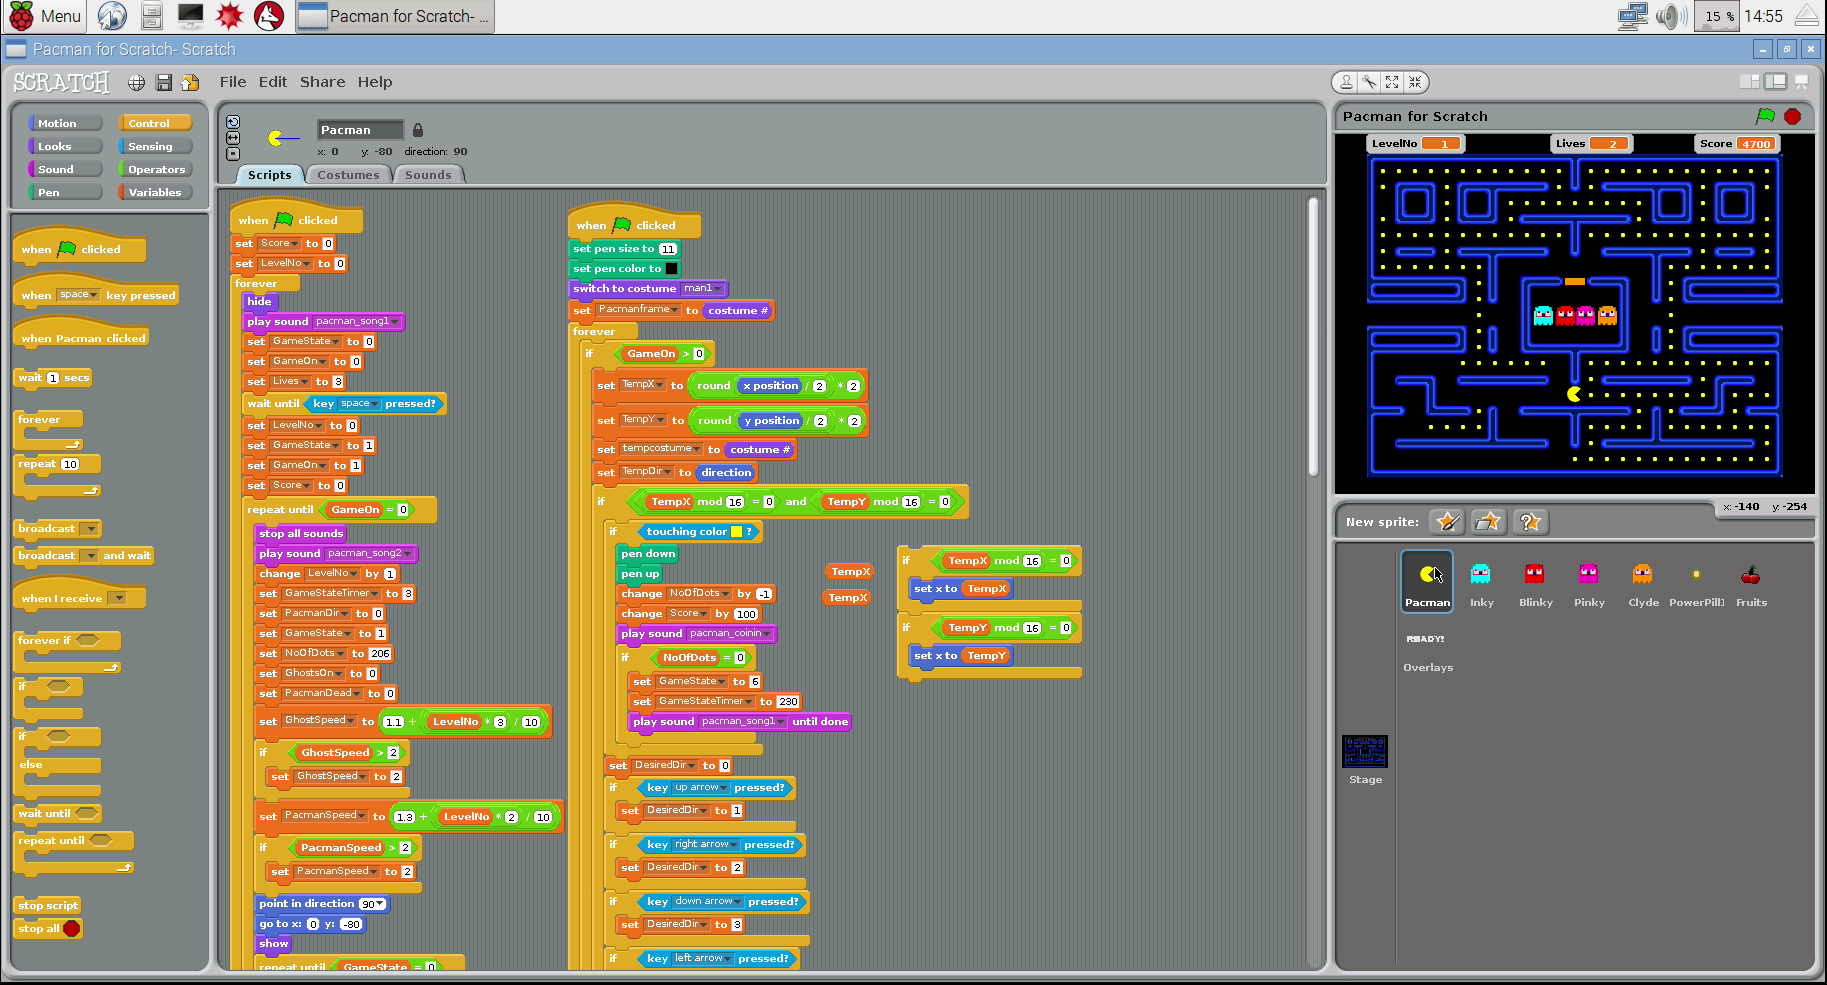
\includegraphics[width=390px]{scratch_rpi.png}
\end{center}

The goal of this coursework is to implement a simple clone of Scratch. Our clone will consist of two components:
\begin{enumerate}
    \item A web-based interface which allows users to construct simple programs visually. This is written in JavaScript and is already implemented for you.
    \item A Haskell program which handles the evaluation of such programs. This is partially implemented and you will have to finish it.
\end{enumerate}
Your task is to complete the part of the Haskell program responsible for evaluating programs -- in other words, you have to write an \emph{interpreter}.

An interpreter is a program which, given some representation of a program as argument, evaluates it. To illustrate this idea, a Haskell implementation of an interpreter for a simple expression language is shown below:
\begin{displaymath}
\begin{array}{l}
\begin{array}{lcl}
\mathbf{data}~\mathit{Expr} & = & \mathit{Val}~\mathit{Int} \mid \mathit{Add}~\mathit{Expr}~\mathit{Expr}
\end{array} \\\\
\begin{array}{lcl}
\mathit{eval} & :: & \mathit{Expr} \to \mathit{Int} \\
\mathit{eval}~(\mathit{Val}~n) & = & n\\
\mathit{eval}~(\mathit{Add}~l~r) & = & \mathit{eval}~l + \mathit{eval}~r
\end{array}
\end{array}
\end{displaymath}
Expressions in the language represented by $\mathit{Expr}$ consist of the addition operator and integer values. The $\mathit{eval}$ function is the interpreter for this language, which determines the value of a given expression.

\subsection*{Getting started}

Clone the skeleton code for this coursework onto your machine:
\begin{verbatim}
$ git clone https://github.com/cs256/cswk2
\end{verbatim}
The code should compile out of the box. You can test this by running:
\begin{verbatim}
$ stack build
\end{verbatim}
To start the program, you should run the following:
\begin{verbatim}
$ stack exec scratch-clone
Starting web server...
Started. Press any key to quit.
\end{verbatim}
In order to view the user interface, open your web browser and navigate to\footnote{If, for whatever reason, port 8000 is unavailable on your machine, you can change this by modifying the definition of $\mathit{main}$ in \texttt{src/Main.hs}.}:
\begin{verbatim}
http://localhost:8000/
\end{verbatim}
You can drag together programs using building blocks from the toolbox on the left. However, if you click ``Evaluate'' at the top right corner of the screen, you will get an error since the interpreter is not yet implemented.

The skeleton code contains a bunch of files, most of which you do not need to touch initially. The most important file is \texttt{src/Interpreter.hs} which contains the definitions you will need to complete to get the interpreter to work. There are some definitions to get you started. A program's initial memory is represented as a list of pairs. Each pair represents one variable, consisting of a name of type $\mathit{String}$ and a value of type $\mathit{Int}$:
\begin{displaymath}
\begin{array}{lcl}
\mathbf{type}~\mathit{Memory} & = & \hslist{(\mathit{String}, \mathit{Int})}
\end{array}
\end{displaymath}
It is possible for things to go wrong when interpreting a program. There are two sorts of errors which may occur. These are represented by the following data type:
\begin{displaymath}
\begin{array}{lcl}
\mathbf{data}~\mathit{Err} & = & \mathit{DivByZeroError} \mid \mathit{UninitialisedMemory}~\mathit{String}
\end{array}
\end{displaymath}
The types representing the language itself are defined in \texttt{src/Language.hs}. You should have a look at this file yourself, but an overview of the most important types is below. A program is a list of statements:
\begin{displaymath}
\begin{array}{lcl}
\mathbf{type}~\mathit{Program} & = & \hslist{\mathit{Stmt}}
\end{array}
\end{displaymath}
There are three different forms of statements: 
\begin{displaymath}
\begin{array}{lcl}
\mathbf{data}~\mathit{Stmt} & = & \mathit{AssignStmt}~\mathit{String}~\mathit{Expr} \\
& \mid & \mathit{IfStmt}~\mathit{Expr}~\hslist{\mathit{Stmt}}~\hslist{(\mathit{Expr},\hslist{\mathit{Stmt}})}~\hslist{\mathit{Stmt}} \\
& \mid & \mathit{RepeatStmt}~\mathit{Expr}~\hslist{\mathit{Stmt}}
\end{array}
\end{displaymath}
Assignments, represented by the $\mathit{AssignStmt}$ constructor, consists of the name of the variable that we are assigning a value to and the expression whose value we should assign to the variable. 

If statements, represented by the $\mathit{IfStmt}$, are more complicated. The first expression is the condition of the ``if'' clause. The list of statements which follows is the code that should be run if the condition is true. The list of pairs of expressions and lists of statements represent ``if else'' clauses. Finally, the last list of statements represents the ``else'' clause.

Repeat statements, represented by the $\mathit{RepeatStmt}$ constructor, consist of an expression which determines how many times the repeat loop should be executed and a list of statements which represent the body of the repeat statement.

There are also three forms of expressions:
\begin{displaymath}
\begin{array}{lcl}
\mathbf{data}~\mathit{Expr} & = & \mathit{ValE}~\mathit{Int} \\
& \mid & \mathit{VarE}~\mathit{String} \\
& \mid & \mathit{BinOpE}~\mathit{Op}~\mathit{Expr}~\mathit{Expr}
\end{array}
\end{displaymath}
The $\mathit{ValE}$ constructor represents integer values, the $\mathit{VarE}$ constructor represents variables, and the $\mathit{BinOpE}$ constructor generalises binary operators. The $\mathit{Op}$ data type in \texttt{src/Language.hs} enumerates all available operators.

\subsection*{Task}

Complete the definition of the $\mathit{interpret}$ function in \texttt{src/Interpreter.hs} so that all values of type $\mathit{Program}$ can be evaluated correctly according to the rules described below. Programs are sequences of statements and should be evaluated in the order in which they are given. We illustrate all rules for the language with screenshots of the GUI and the expected results:

\begin{center}
	\begin{longtable}[t]{|c|p{5cm}|}
		\hline 
		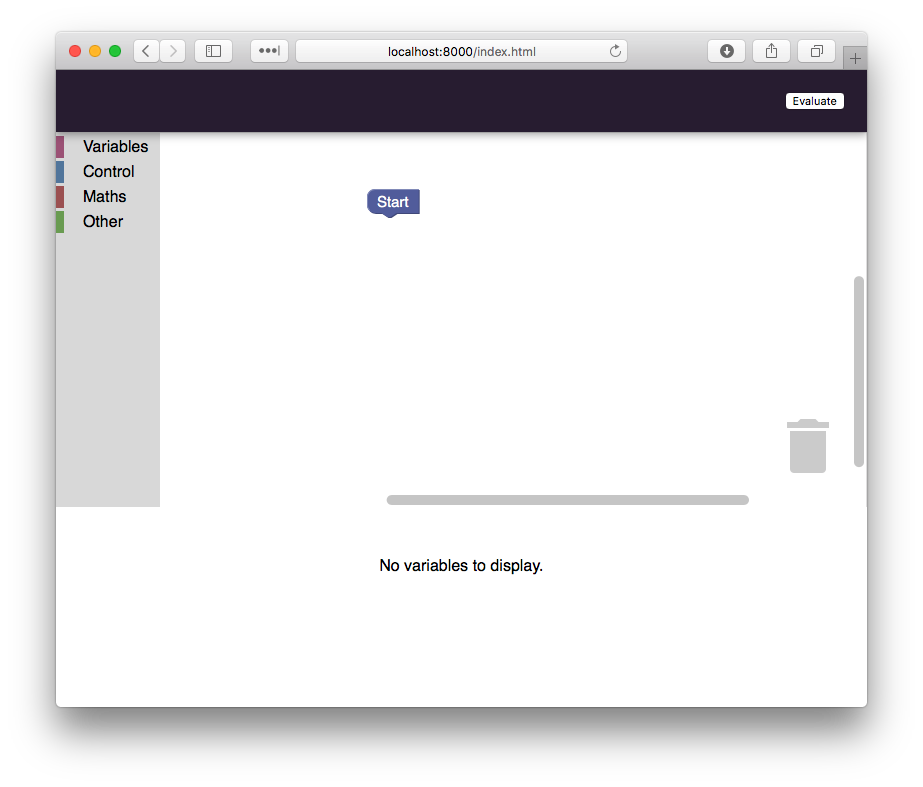
\includegraphics[align=t,width=250px]{semantics/0-empty.png} & 
		If the program is empty as shown in the screenshot, the initial contents of the memory should be returned. \\ \hline 
		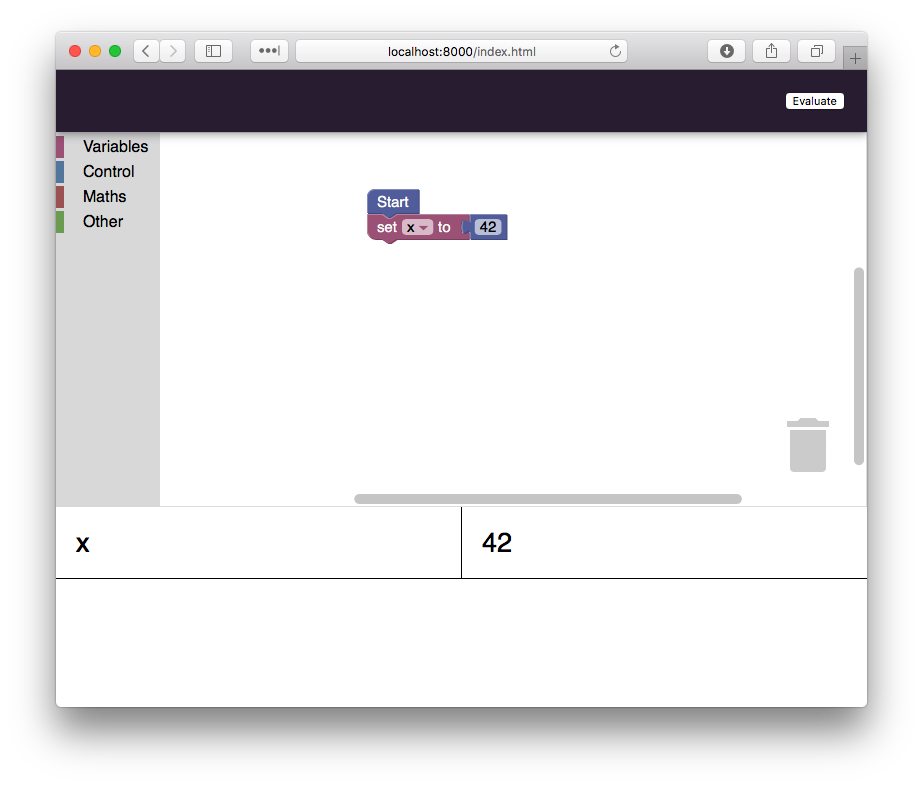
\includegraphics[align=t,width=250px]{semantics/1-assignment.png} & 
		Assignment statements should update the memory to the value of their expression. \\ \hline 
		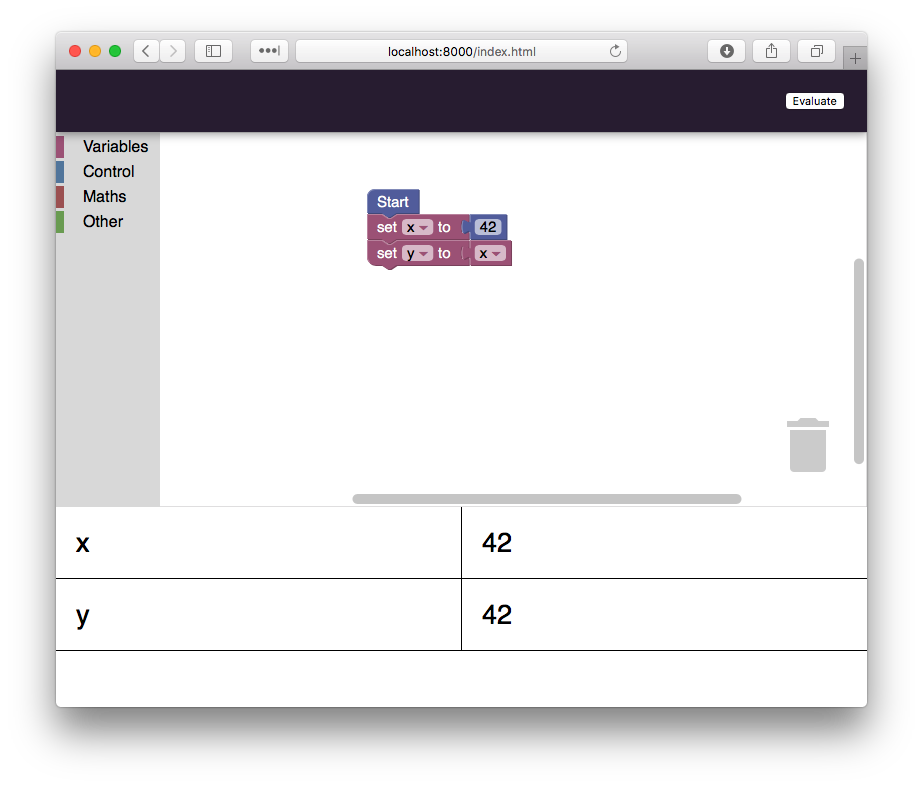
\includegraphics[align=t,width=250px]{semantics/2-loading.png} &
		If a variable occurs in an expression, the corresponding value should be loaded from memory. \\ \hline 
		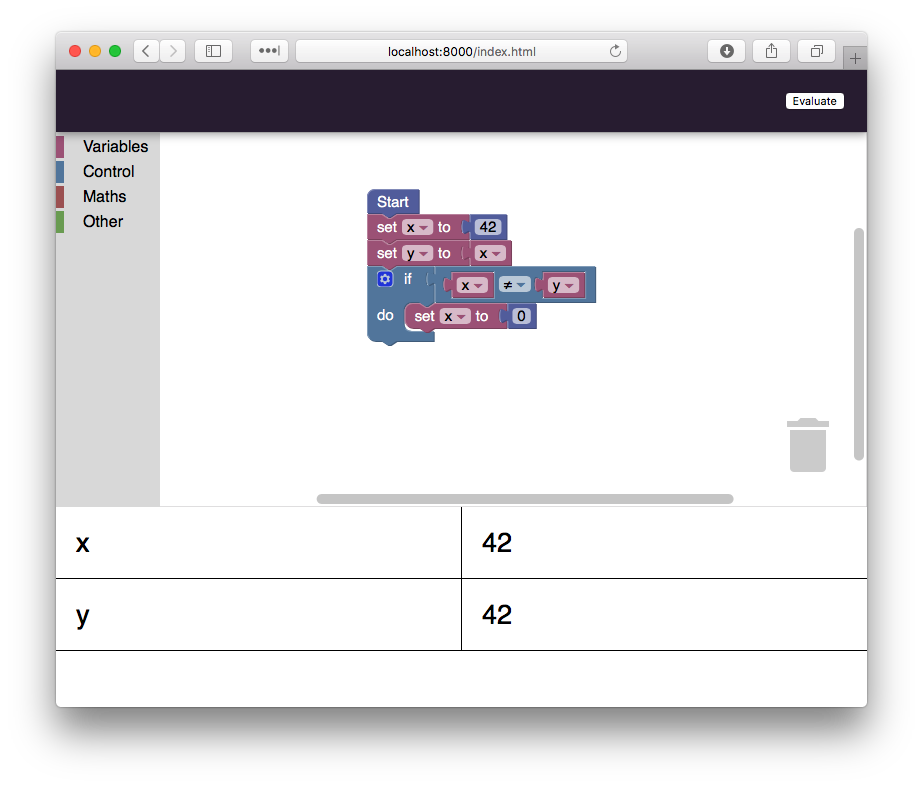
\includegraphics[align=t,width=250px]{semantics/3-if.png} &
		If the condition of an if statement is true (\emph{i.e.} any non-zero value), then the body of the if clause should be executed. \\ \hline
		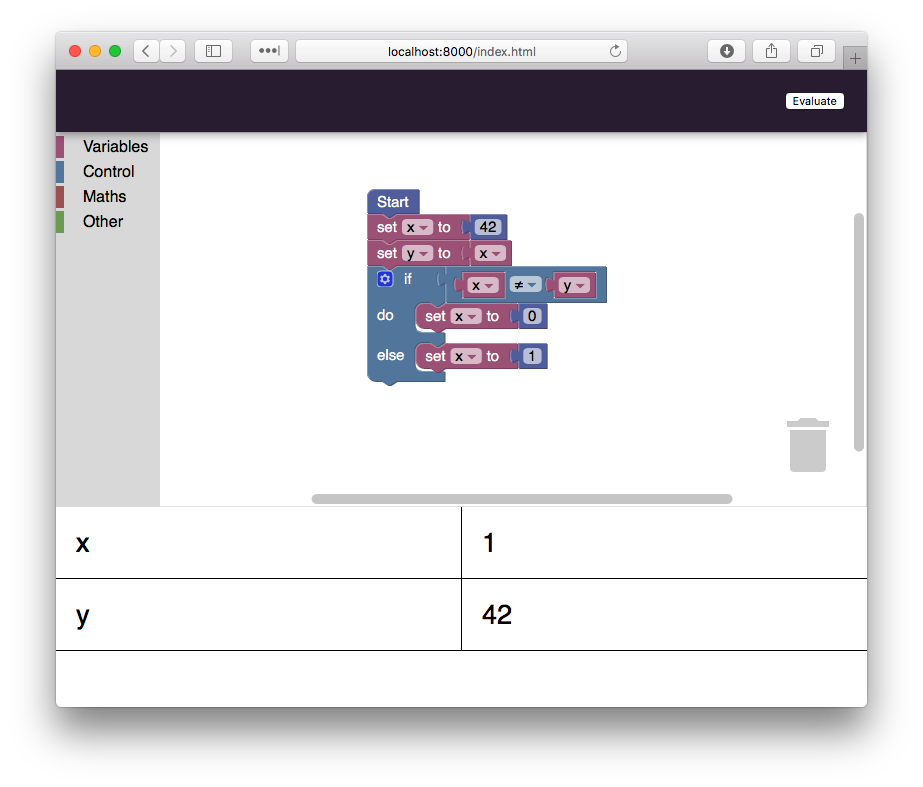
\includegraphics[align=t,width=250px]{semantics/4-else.png} &
		If the condition of an if statement is false (\emph{i.e.} it evaluates to zero), then the body of the else clause should be executed. \\ \hline 
		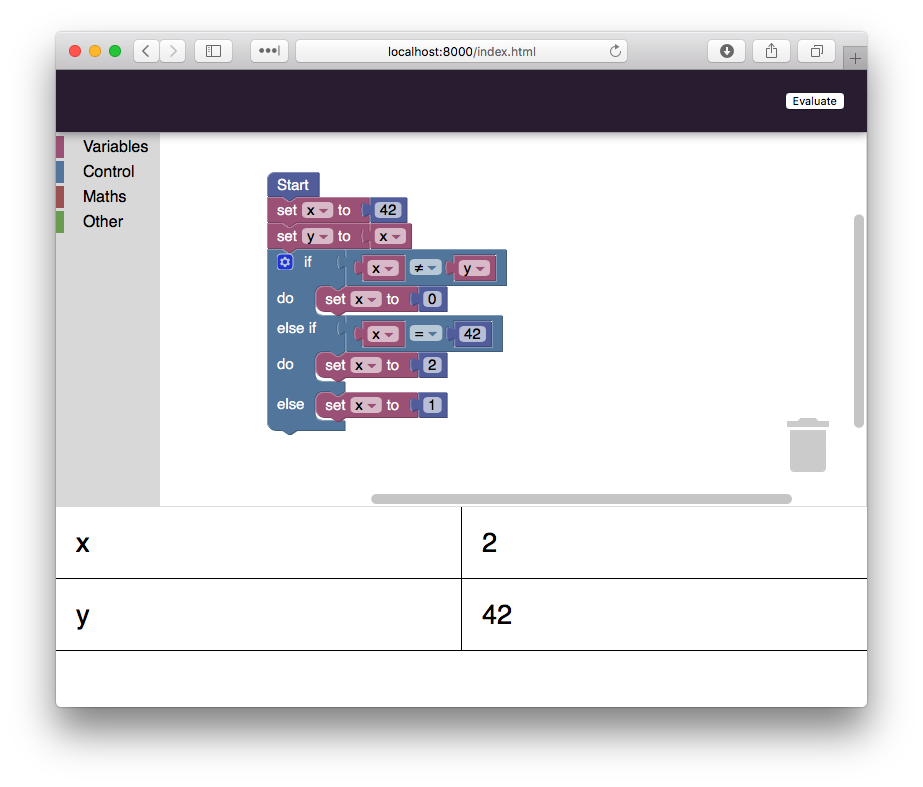
\includegraphics[align=t,width=250px]{semantics/5-ifelse.png} &
		If there are if else clauses present, their conditions should be checked in order after that of the main if clause. If one of them is true, then the corresponding body should be executed. \\ \hline
		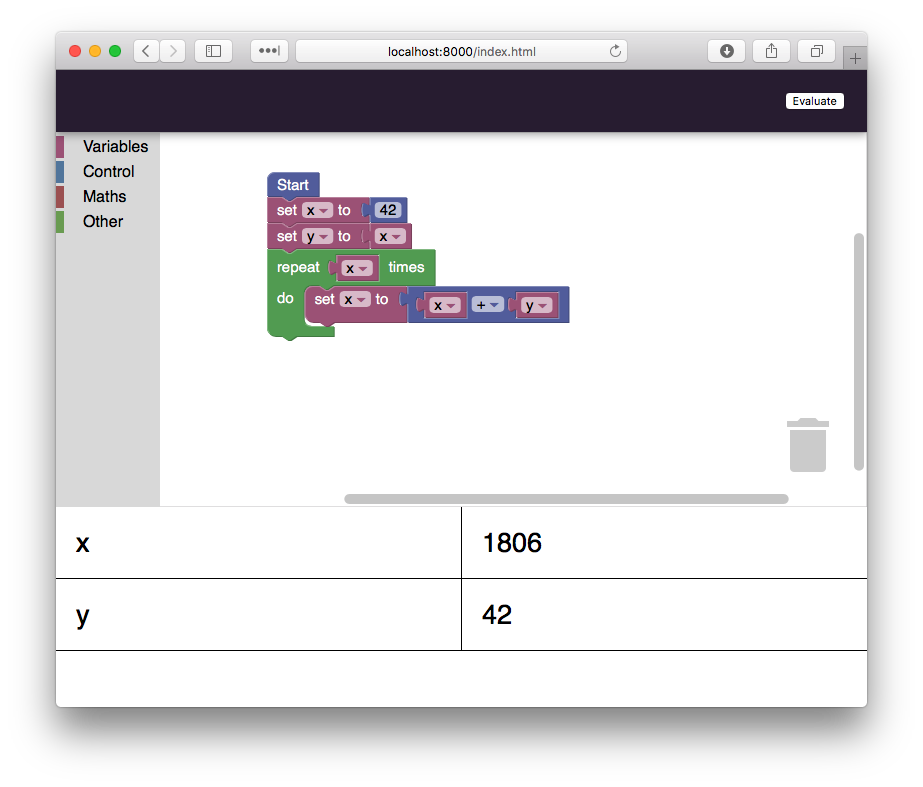
\includegraphics[align=t,width=250px]{semantics/6-repeat.png} &
		Repeat statements evaluate an expression to determine how many times they should run. The body of the repeat statement is then executed that many times. \\ \hline 
		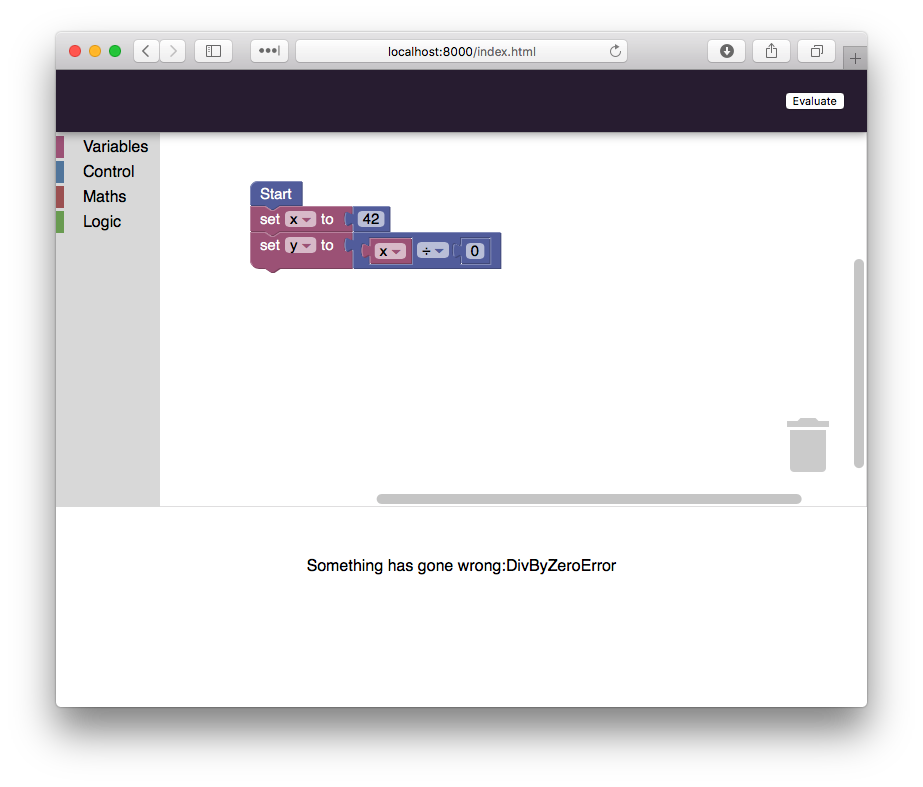
\includegraphics[align=t,width=250px]{semantics/7-divbyzero.png} &
		If a division by zero is attempted, the corresponding error should be returned. \emph{I.e.} \texttt{Left DivByZeroError} \\ \hline
	\end{longtable}
\end{center}
Internally, logic operators should evaluate to $0$ if false and $1$ if true. If an attempt is made to read from a variable which is not in the memory, then the corresponding error should be returned.

Running \texttt{stack test} will give you a rough indication of how complete your solution is. Running \texttt{stack bench} will benchmark your code.

\subsection*{Marking \& submission}

This coursework is worth 25\% of the overall module mark. It will be marked out of 100\% as follows:
\begin{itemize}
	\item 20\% for \emph{correctness}. You gain full marks here if all parts of the coursework have been attempted and are correct. You may use \texttt{stack test} as a rough indication for whether this is the case, but there are some things the unit tests do not test for, so you should construct programs in the scratch clone and ensure that everything works as described.
	\item 20\% for \emph{documented understanding}. You should document your code with comments and explain how it works. You gain full marks if all code is documented and explained sufficiently well so that someone who is unfamiliar with your code can understand it.
	\item 20\% for \emph{elegance}. Definitions should be concise and readable, new functions should be introduced where needed, existing library functions used when applicable, monads used where possible, etc. 
	\item 20\% for \emph{performance and efficiency}. You will do well here if you use sensible data structures and your functions perform as little redundant computation as possible. You can test performance by running \texttt{stack bench} on different versions of your code to see how they compare. 
	\item 20\% for \emph{improvements and extensions}. This is an opportunity for you to demonstrate creativity and advanced understanding. You could achieve this in many different ways, such as adding additional unit tests, functionality, improved algorithms, etc. You may wish to modify \texttt{exe/Main.hs} as well as other source files or even add new ones. You could also prove some properties about your game on paper. The amount of marks awarded will depend on the complexity and creativity of your extension(s) and improvement(s).
\end{itemize}
Submit a \texttt{.zip} or \texttt{.tar.gz} archive of the whole, completed project (not just \texttt{Interpreter.hs}) through Tabula by \deadlineTime\ on \deadlineDate:

\begin{center} 
\url{\submissionURL}
\end{center}

\end{document}